
% ---------------------------------------------------------------------------
% Author guideline and sample document for EG publication using LaTeX2e input
% D.Fellner, v1.20, Jan 18, 2023

\documentclass{egpubl}
\usepackage{STAG2025}

% --- for  Annual CONFERENCE
% \ConferenceSubmission   % uncomment for Conference submission
% \ConferencePaper        % uncomment for (final) Conference Paper
% \STAR                   % uncomment for STAR contribution
% \Tutorial               % uncomment for Tutorial contribution
% \ShortPresentation      % uncomment for (final) Short Conference Presentation
% \Areas                  % uncomment for Areas contribution
% \Education              % uncomment for Education contribution
% \Poster                 % uncomment for Poster contribution
% \DC                     % uncomment for Doctoral Consortium
%
% --- for  CGF Journal
% \JournalSubmission    % uncomment for submission to Computer Graphics Forum
% \JournalPaper         % uncomment for final version of Journal Paper
%
% --- for  CGF Journal: special issue
% \SpecialIssueSubmission    % uncomment for submission to , special issue
% \SpecialIssuePaper         % uncomment for final version of Computer Graphics Forum, special issue
%                          % EuroVis, SGP, Rendering, PG
% --- for  EG Workshop Proceedings
% \WsSubmission      % uncomment for submission to EG Workshop
\WsPaper           % uncomment for final version of EG Workshop contribution
% \WsSubmissionJoint % for joint events, for example ICAT-EGVE
% \WsPaperJoint      % for joint events, for example ICAT-EGVE
% \Expressive        % for SBIM, CAe, NPAR
% \DigitalHeritagePaper
% \PaperL2P          % for events EG only asks for License to Publish

% --- for EuroVis
% for full papers use \SpecialIssuePaper
% \STAREurovis   % for EuroVis additional material
% \EuroVisPoster % for EuroVis additional material
% \EuroVisShort  % for EuroVis additional material
% \MedicalPrize  % uncomment for Medical Prize (Dirk Bartz) contribution, since 2021 part of EuroVis

% Licences: for CGF Journal (EG conf. full papers and STARs, EuroVis conf. full papers and STARs, SR, SGP, PG)
% please choose the correct license
%\CGFStandardLicense
%\CGFccby
%\CGFccbync
%\CGFccbyncnd

% !! *please* don't change anything above
% !! unless you REALLY know what you are doing
% ------------------------------------------------------------------------
\usepackage[T1]{fontenc}
\usepackage{dfadobe}

%\usepackage{cite}  % comment out for biblatex with backend=biber
% ---------------------------
%\biberVersion
\BibtexOrBiblatex
%\usepackage[backend=biber,bibstyle=EG,citestyle=alphabetic,backref=true]{biblatex}
%\addbibresource{egbibsample.bib}
% ---------------------------
\electronicVersion
\PrintedOrElectronic

% for including postscript figures
% mind: package option 'draft' will replace PS figure by a filename within a frame
\ifpdf \usepackage[pdftex]{graphicx} \pdfcompresslevel=9
\else \usepackage[dvips]{graphicx} \fi

\usepackage{egweblnk}
% end of prologue

% ====== OUR DEFS ==========
\usepackage[english]{babel}
\usepackage{amsfonts}
\usepackage{amsmath}
%\usepackage{amsthm}
\usepackage{mathtools}
\usepackage{libertinus}
\usepackage{algpseudocodex}
\usepackage{algorithm}
\usepackage{csquotes}
\usepackage{hyperref}
\usepackage{listings}
\usepackage{xcolor}
\usepackage{float}
\usepackage[capitalize,noabbrev]{cleveref}
\usepackage{tikz-3dplot}

% It seems that libertinus already loads the inconsolata font, so adding the package for that results in a conflict. Specifying the correct font family is enough.\usepackage{natbib}

\renewcommand{\ttdefault}{zi4}

\DeclareMathOperator*{\argmax}{arg\,max}
\DeclareMathOperator*{\argmin}{arg\,min}

\renewcommand{\algorithmicrequire}{\textbf{Input:}}
\renewcommand{\algorithmicensure}{\textbf{Output:}}

\newcommand{\True}{\textsc{true}}
\newcommand{\False}{\textsc{false}}
\newcommand{\EValid}{\textsc{valid}}
\newcommand{\EInvalid}{\textsc{invalid}}
\newcommand{\EUncertain}{\textsc{uncertain}}

\newcommand{\reals}{\mathbb{R}}
\newcommand{\ints}{\mathbb{Z}}
\newcommand{\nats}{\mathbb{N}}
\newcommand{\floor}[1]{\lfloor#1\rfloor}
\newcommand{\ceil}[1]{\lceil#1\rceil}

\newcommand{\intervals}{\mathbb{I}}
\newcommand{\lagpoly}{\mathcal{L}}
\newcommand{\bezpoly}{\mathcal{B}}
\newcommand{\support}{\mathrm{supp}}
\newcommand{\timedep}[1]{\overline{#1}}
\newcommand{\transition}[2]{\mathbf{T}_{#1\to#2}}
\newcommand{\intset}[1]{\mathbb{I}(#1)}
\newcommand{\indexset}{\mathcal{I}}
\newcommand{\cornerset}{\mathcal{C}}
\newcommand{\domainpts}{\Gamma}
\newcommand{\intlo}[1]{{[#1]}_{\textrm{lo}}}
\newcommand{\inthi}[1]{{[#1]}_{\textrm{hi}}}
\newcommand{\lowend}[1]{\underline{#1}}
\newcommand{\upend}[1]{\overline{#1}}
\newcommand{\inclusion}[1]{\Box #1}
\newcommand{\minclusion}[1]{\Box_{\min} #1}
\newcommand{\sampleset}[1]{\mathcal{S}_{#1}}
\newcommand{\polyspace}[2]{\mathcal{P}_#1^#2}

\newcommand{\solve}{\textsc{Solve}}
\newcommand{\minimize}{\textsc{Minimize}}
%\newcommand{\keyword}[1]{\texttt{#1}}

\newtheorem{theorem}{Theorem}
\newtheorem{lemma}{Lemma}
\newtheorem{definition}{Definition}

%------------------------------------------------------------------------ % Alter some LaTeX defaults for better treatment of figures: 
% See p.105 of "TeX Unbound" for suggested values. 
% See pp. 199-200 of Lamport's "LaTeX" book for details. % General parameters, for ALL pages:
\renewcommand{\topfraction}{0.9} % max fraction of floats at top 
\renewcommand{\bottomfraction}{0.8} % max fraction of floats at bottom 
% Parameters for TEXT pages (not float pages): 
\setcounter{topnumber}{4} 
\setcounter{bottomnumber}{4} 
\setcounter{totalnumber}{8} % 2 may work better 
\setcounter{dbltopnumber}{4} % for 2-column pages 
\renewcommand{\dbltopfraction}{0.95} % fit big float above 2-col. text 
\renewcommand{\textfraction}{0.07} % allow minimal text w. figs % Parameters for FLOAT pages (not text pages): 
\renewcommand{\floatpagefraction}{0.7} % require fuller float pages % N.B.: floatpagefraction MUST be less than topfraction !! 
\renewcommand{\dblfloatpagefraction}{0.7} % require fuller float pages %------------------------------------------------------------------------

% CONFIGURATION OF listings
\definecolor{codegreen}{rgb}{0,0.6,0}
\definecolor{codegray}{rgb}{0.5,0.5,0.5}
\definecolor{codepurple}{rgb}{0.58,0,0.82}
\definecolor{backcolour}{rgb}{0.95,0.95,0.92}


\lstdefinestyle{smallcode}{
    backgroundcolor=\color{backcolour}, 
    commentstyle=\color{codegreen},
    keywordstyle=\color{magenta},
    keywordstyle=[3]\color{red},
    numberstyle=\tiny\color{codegray},
    stringstyle=\color{codepurple},
    basicstyle=\ttfamily\tiny,
    breakatwhitespace=false,
    breaklines=true,
    captionpos=b,
    numbers=left,
    numbersep=5pt,
    tabsize=2,
}

\lstdefinestyle{largecode}{
    style=smallcode,
    basicstyle=\ttfamily\scriptsize,
    numbers=none,
}

\lstdefinelanguage{miso}{
    language=Python, % inherit Python syntax
    deletekeywords=[2]{sum},
    morekeywords={with, as, assert},
    morekeywords=[3]{variables, arguments, poly_space, geo_map, bases, collapse, expand, subdiv_strategy, generate, Context, vector, basis, jacobian, det, sum, prod},
}


\lstset{style=smallcode}
% END listings

\title[Short title here]%
      {\emph{TIGHT} Intervals for Provably Correct Geometric Computation}

% for anonymous conference submission please enter your SUBMISSION ID
% instead of the author's name (and leave the affiliation blank) !!
% for final version: please provide your *own* ORCID in the brackets following \orcid; see https://orcid.org/ for more details.
\author[Anonymous]
{\parbox{\textwidth}{\centering Anonymous authors}}
%{\parbox{\textwidth}{\centering D.\,W. Fellner\thanks{Chairman Eurographics Publications Board}$^{1,2}$\orcid{0000-0001-7756-0901}
 %       and S. Behnke$^{2}$\orcid{0000-0001-5923-423X}
%        S. Spencer$^2$\thanks{Chairman Siggraph Publications Board}
%        }
%       \\
% For Computer Graphics Forum: Please use the abbreviation of your first name.
%{\parbox{\textwidth}{\centering $^1$TU Darmstadt \& Fraunhofer IGD, Germany\\
 %        $^2$Graz University of Technology, Institute of Computer Graphics and Knowledge Visualization, Austria
%        $^2$ Another Department to illustrate the use in papers from authors
%             with different affiliations
%       }
%}
%}
% ------------------------------------------------------------------------

% if the Editors-in-Chief have given you the data, you may uncomment
% the following five lines and insert it here
%
% \volume{36}   % the volume in which the issue will be published;
% \issue{1}     % the issue number of the publication
% \pStartPage{1}      % set starting page


%-------------------------------------------------------------------------
\begin{document}

\teaser{
 
\includegraphics[width=0.4\linewidth]{fig/512x512.png}
 \centering
  \caption{this is the teaser}
\label{fig:teaser}
}

\maketitle
%-------------------------------------------------------------------------
\begin{abstract}
Interval arithmetic is a practical method for robust computation, bridging the gap between \FS{fast but} inexact floating-point arithmetic and slow, exact arithmetic (such as rational or arbitrary-precision). In this system, numbers are represented as intervals bounded by floating-point numbers. Operations are performed conservatively, guaranteeing that the resulting interval contains the exact mathematical result.

%We present a new C++ library for interval arithmetic that supports both algebraic and transcendental functions. A key feature of this library is its use of correctly rounded operations, ensuring the resulting interval is the smallest floating-point interval that contains the true result.
\FS{We extend a fast C++ library for interval arithmetic with a wide set of common mathematical functions. A key feature of our library is that its operations are correctly rounded, ensuring the resulting interval is the smallest floating-point interval that contains the true result.}
We demonstrate the library’s effectiveness by applying it to complex non-polynomial problems, including continuous collision detection for geometric primitives undergoing roto-translational motion.
%-------------------------------------------------------------------------
%  ACM CCS 1998
%  (see https://www.acm.org/publications/computing-classification-system/1998)
% \begin{classification} % according to https://www.acm.org/publications/computing-classification-system/1998
% \CCScat{Computer Graphics}{I.3.3}{Picture/Image Generation}{Line and curve generation}
% \end{classification}
%-------------------------------------------------------------------------
%  ACM CCS 2012
%  (see https://www.acm.org/publications/class-2012)
%The tool at \url{http://dl.acm.org/ccs.cfm} can be used to generate
% CCS codes.
%Example:
\begin{CCSXML}
<ccs2012>
<concept>
<concept_id>10010147.10010371.10010352.10010381</concept_id>
<concept_desc>Computing methodologies~Collision detection</concept_desc>
<concept_significance>300</concept_significance>
</concept>
<concept>
<concept_id>10010583.10010588.10010559</concept_id>
<concept_desc>Hardware~Sensors and actuators</concept_desc>
<concept_significance>300</concept_significance>
</concept>
<concept>
<concept_id>10010583.10010584.10010587</concept_id>
<concept_desc>Hardware~PCB design and layout</concept_desc>
<concept_significance>100</concept_significance>
</concept>
</ccs2012>
\end{CCSXML}

\ccsdesc[300]{Computing methodologies~Collision detection}
\ccsdesc[300]{Hardware~Sensors and actuators}
\ccsdesc[100]{Hardware~PCB design and layout}


\printccsdesc
\end{abstract}
%-------------------------------------------------------------------------

% !TEX root = STAG25-MiSo2.tex

\section{Introduction}
\label{sec:introduction}
Robust geometric computation is a critical component of many applications, such as collision detection, minimum distance computation, element inversion, and Boolean operations \cite{something}. Although floating-point arithmetic is fast, it can easily generate inaccurate results that may lead to unpredictable, often catastrophic outcomes, especially in simulations \cite{something}. In contrast, exact computation, using methods like rational arithmetic or arbitrary precision floating-point arithmetic, is extremely slow and often impractical.
Moreover, such methods are exact only for algebraic operations. 

Interval arithmetic bridges this gap by providing a viable alternative. 
It offers a balance between performance and accuracy, giving conservative estimates of exact computations at a moderate speed penalty compared to standard floating-point arithmetic. In this model, all real values are represented as intervals bounded by floating-point numbers. Expressions on these intervals are computed in a way that guarantees the resulting interval will contain the true mathematical result.
While the width of an interval can grow during computation, it is crucial to minimize this growth to maintain precision. This is achieved through \emph{correctly rounded} operations, where each elementary operation returns the tightest possible floating-point interval that contains the exact result.
%More fundamentally, if elementary computations are not correctly rounded, the same expression %evaluated with the same sequence of operations
% may give different results on different architectures, or even on the same architecture once the underlying mathematical library is changed. 

The IEEE 754 standard prescribes correctly rounded results only for the algebraic operations and the square root; all other 
%transcendental
operations are just \emph{recommended} to be correctly rounded, but there is no guarantee, depending on their implementation.
%The CORE-MATH project \cite{core-math} provides correctly rounded implementations for all the most common transcendental operations. 
Consequently, nowadays no libraries exist that guarantee the creation of as-tight-as-possible intervals when the expressions involve this kind of operations.
See Section \ref{sec:related} for further discussion.

% TOLTA FRASE SEGUENTE, RIPETE LE PRIMA DELL'INTRO
%Since such a kind of expressions are useful in diverse graphics applications (e.g., non-linear element inversion, collision detection, Boolean operations), i
In this paper, we describe the design principles of our TIGHT library for interval arithmetic, which always produces as-tight-as-possible intervals, is faster than any existing library, and supports transcendental functions.
%
Our original contributions include:
\begin{enumerate}
\item We extend the NFG library \cite{nfg} -- which provides the most efficient implementation of interval arithmetic to date, but is limited to algebraic operations -- with transcendental operations, based on the CORE-MATH floating-point correctly rounded implementation \cite{Sibidanov2022}.
In Section \ref{sec:functions}, we discuss the challenges involved in extending transcendental operators to intervals while guaranteeing correct rounding. 
\item We integrate our library with the recent Domain Specific Language MiSo \cite{Sichetti2025} that supports the fast prototyping of non-linear constraint solving and optimization. 
Extension of the language with transcendental functions largely broadens its spectrum of applicability. 
\item We demonstrate the effectiveness and efficiency of our library by implementing surface-surface intersection between non-algebraic surfaces, and continuous collision detection between geometric primitives undergoing roto-translational motion.  We also compare our library against the Filib library \cite{filib}, achieving a faster performance.
\end{enumerate}


%THE REST IS FROM SIGGRAPH PAPER - PROBABLY OBSOLETE, MAYBE SOMETHING USEFUL FOR THE RELATED

%Non-linear constraint solving is fundamental to graphics and scientific computing, with applications ranging from collision detection and minimal distance computation to element inversion and Boolean operations. A vast literature addresses this topic (Section \ref{sec:related}). For example, \cite{RTR4,Akenine2024} summarize methods for static collision detection between proxies, referencing over 100 algorithms tailored to different primitive pairs and accuracy/efficiency trade-offs.
%Similar per-primitive-pair specialization is required for minimal distance queries and, likewise, each finite element (FE) type and order necessitates custom code for positive Jacobian checks.
%This complexity doubles when considering time-dependent scenarios.

%While real-time applications often restrict primitives to boxes due to limited computational resources, high-fidelity simulations may require conservative, high-accuracy predicates \cite{snyder92}.
%Testing the correctness and ensuring the efficient, accurate implementation of these algorithms is a major challenge \cite{Wang2021}. The difficulty of generalizing theoretical improvements across different cases hinders progress in this pervasive and crucial family of algorithms, essential to modern computing.

%In contrast to algorithm specialization, Snyder \cite{snyder92} proposed a general framework, based on interval analysis, for conservative solutions to high-order constrained optimization. This framework offers two algorithms: \solve, which finds all solutions to a non-linear constraint system, and \minimize, which finds the constrained global minimum of a function. For \solve, the conservative algorithm returns a region guaranteed to contain all solutions (if any), potentially including points near the feasible domain. For \minimize, it returns a value less than or equal to the true minimum and within a bounded distance of it. In both cases, this conservativeness accounts for numerical rounding errors.

%Although often considered slower than methods like Newton's minimization, recent work \cite{Wang2021,Chen2024} 
 %demonstrates the effectiveness and relative efficiency of this conservative approach, particularly when seeking guaranteed solutions. 

%Snyder's approach uses Natural Interval Extensions (NIE) to compute \emph{inclusion functions} (\cref{sub:inclusion}) that bound function ranges over domains, by composition of interval operators (\cref{app:interval}). Although general, NIE's convergence to the true range via domain decomposition can be slow. 
%For the common case of polynomials, tighter bounds are achievable via their Bézier representation \cite{Lengagne:2020,stahl_interval_1995,johnen2013}. 
%However, Bézier representation can be computationally expensive for polynomials with many terms. 

%We employ a hybrid approach, blending Bézier inclusion functions and NIE. Decomposing polynomial expressions into simpler forms (fewer variables or lower degree) allows us to construct a spectrum of inclusion functions that ranges from fully NIE-based (expanded expressions) to fully Bézier-based (collapsed expressions).
%Hybrid solutions can dramatically improve efficiency. For example, our hybrid solver for continuous collision detection between high-order polynomial patches is orders of magnitude faster than purely NIE-based and purely Bézier-based solutions (\cref{sec:results}).

%We developed MiSo on top of such a hybrid approach. MiSo is a Python-based domain-specific language (DSL) for the specification of \solve\ and \minimize\ problems. MiSo enables the user to quickly explore possible hybrid approaches by changing a few lines of code.
%From a simple specification, the MiSo compiler produces a numerically robust C++ solver for the given problem, automatically generating all the necessary representations of the functions involved, the related transformations required for domain subdivision, and the evaluation of inclusion functions.

%Domain decomposition and interval arithmetic are used to guarantee conservative results. Setting a compile-time flag switches to a faster, non-conservative computation mode based on standard floating-point arithmetic.
%A known limitation of subdivision-based methods is that they suffer from a curse of dimensionality; hence, our method may become impractical for problems in many dimensions. However, we show that we are able to achieve competitive performance for a number of fundamental geometric problems, especially those involving high-order geometry.

%We demonstrate competitive performance against hand-optimized code for key computer graphics problems, including linear and high-order continuous collision detection, and finite element validity checks.

%MiSo is available as an open-source project at \url{https://gitlab.com/fsichetti/miso}.


% !TEX root = STAG25-MiSo2.tex

\section{Background and state of the art}
\label{sec:related}

Interval arithmetic \cite{hickey2001} provides a set of operations on real intervals $\intervals$ such that if $x\in a=[\intlo{a},\inthi{a}] \in \intervals$ and $y\in b=[\intlo{b},\inthi{b}] \in \intervals$,
then $x \star y  \in a \star b$, where $\star$ in the right-hand side is the interval version of operation $\star$ on reals.
We are interested in intervals whose lower and upper bounds can be represented by FP numbers.

From now on, the set of representable FP numbers is denoted by $\mathbb{F}$. When $a$ and $b$ are in $\mathbb{F}$, the result $r = a \star b$ may be not in $\mathbb{F}$, and hence not representable. In that case $i=[fp^{-}(r),fp^{+}(r)]$, where $fp^{-}(r) = max(f : f \in \mathbb{F}, f \leq r)$ and $fp^{+}(r) = min(f : f \in \mathbb{F})$, is the tightest representable interval containing $r$.
IEEE 754 requires that when $\star$ is an algebraic operation (or the square root) an implementation of $\star$ must round the theoretically exact result $r$ to either $fp^{-}(r)$ or $fp^{+}(r)$, depending on the current \emph{rounding mode}.
In most modern architectures the rounding mode is controlled by a particular register within the CPU, and specific system functions exist to set it. Therefore, a trivial approach to create a tight interval for the operation $a \star b$ is to (1) set the rounding mode to $towards -\infty$, (2) execute $a \star b$ to determine the interval's lower bound, (3) set the rounding mode to $towards +\infty$, (4) execute $a \star b$ to determine the interval's upper bound.
Since setting the rounding mode is typically slower than executing arithmetic operations, a more efficient approach is (1) set the rounding mode to $towards +\infty$, (2) execute $(-a) \star b$ and switch the sign of the result to determine the interval's lower bound, (3) execute $a \star b$ to determine the interval's upper bound. Furthermore, if no other parts of the program require a different rounding, step (1) can be executed only once at the beginning.
This approach is used by existing interval arithmetic libraries such as Boost \cite{bronnimann2006} and CGAL \cite{cgal}.

Another possibility is to deconstruct the binary representation of the result $r$ to directly modify the mantissa, exponent and sign, and produce a reasonably small interval around $r$. This approach is used by Filib and some modes of Filib++ \cite{filib, filibpp}.
Alternatively, the error propagation can be analyzed to derive a bound $\epsilon$ on the rounding so that the interval $i=[r-\epsilon,r+\epsilon]$ is guaranteed to contain $r$. This is how libraries such as BIAS \cite{bias} or GAOL \cite{gaol} work.

The aforementioned existing libraries were comprehensively compared by Tang and colleagues \cite{tang2022} who evaluated diverse aspects, including their correctness, efficiency and precision (in terms of interval tightness). Their conclusion is that only filib and filib++ are always correct when transcendental functions are involved, although the intervals they produce might be larger than necessary. In contrast, Boost and BIAS may produce intervals that do not contain the exact result. Also, Tang's evaluation could verify that libraries that use the rounding mode produce tighter intervals.

With the exception of rather old architectures, most existing CPUs provide SIMD registers and instructions that proved useful to accelerate interval arithmetic libraries \cite{lambov2008}. Here the basic idea is to store both the bounds in a single 128bit-wide register and perform operations on both bounds in parallel. This and other optimizations exploiting more recent AVX architectures were  included in the NFG library \cite{nfg} that, to the best of our knowledge, represents the fastest existing library at the time of writing. Since NFG exploits the rounding mode, it is also guaranteed to produce as-tight-as-possible intervals for all the algebraic operations and the square root. Our TIGHT library wraps around NFG while adding many other elementary and transcendental functions while keeping the guarantee to produce tight intervals.

\subsection{Correct rounding}
\emph{Correct rounding} refers to the property that an implementation
of a mathematical function $f$ has if, for any $x$ that is representable and contained in the domain of $f$, it returns the same results one would get by rounding the exact result $f(x)$ to the target representation.
%MOVED TO INTRO
%The 2019 revision of the IEEE 754 standard for floating point arithmetic requires a compliant implementation of a function to round correctly for all inputs \cite{ieee}. Indeed, required operations such as summation, subtraction, multiplication, division, and square roots produce the same, correctly rounded results on any IEEE 754-compliant machine. \cite{ieee754}
%However, this is not true for \emph{recommended} functions like $\sin$ or $\log$: because they are not mandatory, mathematical libraries are allowed to implement fast, non-CR routines that are not IEEE 754-conforming, but the language implementation as a whole will be conforming as long as the mandatory operations are CR.

Producing efficient CR implementations of functions is a difficult task that has been actively researched for many years.
The classical method involves performing a fast approximation of the function with a known error bound, followed by a correctness check, and a slower but higher-accuracy approximation if the check fails.
Interestingly, implementing CR double-precision functions is more difficult than single-precision, because one can check correct rounding exhaustively on 32-bit floats, which is infeasible in the 64-bit case.
For double precision, correctness must either be proved formally or tested on known hard to round cases.

The most notable libraries for CR mathematical functions are CRlibm \cite{crlibm} and RLibm \cite{rlibm}.
CRlibm implements several transcendental functions of one double-precision argument, correctly rounded in the four rounding modes. However, instead of following the rounding mode set on the FPU by the user, it provides separate functions for each rounding mode, and it assumes that the FPU is set to round-to-even (whereas interval arithmetic uses directed rounding).
%, and also assumes that the FPU uses double precision internally, whereas double-extended precision is the default on some platforms.
To the best of our knowledge, the project is no longer actively maintained.
RLibm is a more recent project that proposes a new approach to correct rounding by polynomial approximants, but it is currently limited to single-precision inputs.

The CORE-MATH Project \cite{coremath} is an ongoing effort to build a complete collection of correctly rounded C implementations of mathematical functions to foster integration into existing mathematical libraries. CORE-MATH is actively developed and provides efficient CR routines for univariate and bivariate functions with double-precision arguments.

TIGHT uses CORE-MATH functions in its interval extensions for all those functions that are not CR in the C++ standard library.
Because CORE-MATH is not a library proper, we also provide a publicly available C++ wrapper to facilitate its use in projects such as TIGHT: \url{url://omitted.for.anonimity}.

% !TEX root = STAG25-MiSo2.tex

\section{Implementing elementary functions}
\label{sec:functions}
In order to implement robust, conservative and tight interval extensions of elementary functions, we rely on existing \emph{correctly rounded} implementations of functions.
The CORE-MATH Project \cite{Sibidanov2022} provides a collection of fast, correctly rounded implementations of most commonly used mathematical functions.
For ease of use, we created a minimal C++ library of double-precision CORE-MATH implementations that is publicly available at \url{}.

The functions that we implemented are:
\begin{itemize}
	\item
\end{itemize}

\subsection{Interval extension}
Assuming the availability of a correctly rounded function $f$, we want to obtain a correctly rounded inclusion function for $f$, that is, an interval-valued function $\inclusion{f}$ such that the endpoints of the resulting interval are correctly rounded outward.

TIGHT's interval class wraps the NFG interval library \cite{nfg}, which guarantees that the result of every operation contains the true result, thanks to conservative outward rounding. Specifically, the library is initialized by setting the FPU rounding mode to upward, and the lower end of the interval is represented internally with opposite sign, which results in downward rounding without changing the rounding mode.

An issue that must be considered is how to deal with input intervals containing points outside the domain of $f$. We discuss this in Section \ref{}, and until them, we limit our discussion to identifying such ill-posed inputs.

The challenge of extending a function to intervals with correct rounding is twofold.
First, one needs to know the expressions for the endpoints of the resulting interval; this is done by enumerating the possible cases for a given function.
Then, these expressions must be instantiated on the input datum and rounded correctly - downward for the lower bound and upward for the upper one.

\subsubsection{Odd and monotonic functions}
When $f$ is monotonically increasing on $[\intlo{x}, \inthi{x}]$, the image of the interval can be easily computed as $\inclusion{f}([\intlo{x}, \inthi{x}]) = [f(\intlo{x}), f(\inthi{x})]$; if it is monotonically decreasing, the two endpoints are swapped. In both cases, assuming exact arithmetic, the result is exact.
If $f$ is not monotonic on $[\intlo{x}, \inthi{x}]$, we need to know where $f$ attains its extrema on the interval. As we will see for some non-monotonic functions, even deciding that $[\intlo{x}, \inthi{x}]$ is in a monotonic region of the domain is tricky in inexact arithmetic.

Once one knows how to compute the range of the function in exact arithmetic, correct rounding amounts to rounding the left endpoint down, and the right endpoint up. Given that we are operating in round-upward mode, the latter is free. To round down we could change the rounding mode and reset it after the operation.
However, changing roundind modes flushes the CPU pipeline, thus it is an expensive operation that we avoid.
When $f$ is odd, the result of $f(x)$ rounded down is easily computed in upward rounding mode as $-f(-x)$, since negation is an exact operation. Several elementary functions are odd, so this property is helpful for our purposes.

\subsubsection{List of functions}
For a monotonically increasing and odd function $f$, computing $\inclusion{f}$ with upward rounding is as easy as $\inclusion{f}([\intlo{x}, \inthi{x}]) = [-f(-\intlo{x}), f(\inthi{x})]$. Fortunately, many of the functions of interest to us satisfy both these properties:
\FS{TODO}

\subsubsection{Inverse trigonometric, exponential and logarithmic functions}
When we drop the oddity assumption, we face the problem of how to round down the result of a call to the correctly-rounded library function without changing the rounding mode, since doing so incurs a performance penalty.
An easy way to deal with this is to compute the result with upward rounding, then correcting this by taking the immediately preceding FP value.
However, if the exact result of the function is representable as a floating point number, correct rounding imposes that the exact result will be returned; in these special cases, if use the immediately smaller FP value, we get an error of 1 ULP.
To address this, we would like to only perform this operation if the upward rounding happened. Unfortunately, while the IEEE754 standard does provide a way to check this via status flags, CORE-MATH currently does not guarantee that status flags are set correctly.
For many functions it is possible, however, to check \emph{a priori} if the result will be exactly representable as a floating point number, and round down when it is not.

\FS{\dots}

\subsection{Points outside the domain}

%% !TEX root = STAG25-MiSo2.tex

\section{Results and comparison}
\label{sec:results}
We evaluate our library in several scenarios. Furthermore, because Filib/Filib++ is the only library which is always correct when transcendental functions are involved \cite{tang2022}, we compare TIGHT with this representative of the state of the art.

All experiments were timed single-threaded on a server equipped with Intel Xeon Gold 6430 CPUs and 64GB of RAM.
The compiler used is GCC version 13.3.0 on Ubuntu.

\subsection{Benchmark comparison}
We start by comparing the execution times and average interval width of single functions in TIGHT and Filib++.
To compute the width, for each operation we select one or two singleton input intervals that lie inside the function domain, and compute the number of floating point values between the lower and upper ends of the computed interval (plus one); a width of 1 ULP (or 0, in the case of an exactly representable output) corresponds to a correctly rounded result.
To get timings, we call each function one million times; to prevent the compiler from optimizing calls, and to evaluate the timing on non-singleton intervals, we perturb the input interval at each iteration by enlarging it by an ULP on both sides, and sum the upper and lower bound of each result to a dummy accumulator.
Note that some operations are omitted for Filib++ as they are not supported in the library.

Estimated times for executing one interval operation with the two libraries are reported in Table \ref{table:benchmarks}. 
Times are in nanoseconds. 
Note that, for the simplest operations that cost about or even less than one nanosecond, estimates are not fully reliable and may change on different runs.  
The values reported in the table for those operations are averages over different runs. 
However, we consistently had at all runs faster times with TIGHT, for all those operations that are already supported in NFG.   
For the newly implemented transcendental functions, times are comparable, but sometimes they are slower with TIGHT.
This is the cost of all additional operations that we undergo to guarantee correct rounding, which is not guaranteed by Filib++.

The latter issue is evident by looking at the two rightmost columns in Table \ref{table:benchmarks}, which report the width of the resulting interval in ULPs (number of contiguous floating-point values), when the input consists of a singleton $[x,x]$.
While TIGHT always produces intervals with a width of either zero or one ULP, hence correctly rounded, Filib++ produces quite large intervals in many cases (it is still correctly rounded, but slower, for algebraic operations). 

\clearpage
\onecolumn
\begingroup

\tiny
\begin{longtable}{lrrrrrrrrr}
\hline
& Filib & Boost & FL++ NS & FL++ ND & FL++ NOG & FL++ Mul & FL++ PS & TIGHT & FP baseline \\
\hline
ADDITION & 139.841000 & 451.849000 & 77.454000 & 56.244000 & 16.264000 & 46.557000 & 58.725000 & 5.904000 & 5.912000 \\
SUBTRACTION & 135.853000 & 451.776000 & 77.444000 & 56.186000 & 16.295000 & 40.737000 & 58.831000 & 5.914000 & 5.911000 \\
MULTIPLICATION & 153.026000 & 454.497000 & 80.465000 & 58.602000 & 17.472000 & 64.090000 & 86.292000 & 11.230000 & 5.898000 \\
DIVISION & 148.818000 & 448.056000 & 98.105000 & 74.635000 & 37.021000 & 61.618000 & 82.163000 & 47.171000 & 11.826000 \\
SQUARE ROOT & 159.648000 & 447.951000 & 79.588000 & 63.828000 & 46.856000 & 60.580000 & 96.586000 & 35.396000 & 23.587000 \\
EXPONENTIAL & 257.656000 & 449.746000 & 254.173000 & 251.163000 & 205.657000 & 219.957000 & 246.876000 & 178.049000 & 57.764000 \\
SIN & 289.798000 & 1453.097000 & 327.376000 & 324.451000 & 207.906000 & 220.579000 & 233.763000 & 1971.934000 & 317.734000 \\
COS & 288.131000 & 1304.546000 & 324.974000 & 321.932000 & 207.339000 & 221.081000 & 230.165000 & 1943.731000 & 321.314000 \\
ARITHMETIC EXPRESSION 1 & 800.244000 & 2238.724000 & 569.425000 & 506.251000 & 229.616000 & 606.002000 & 757.993000 & 293.389000 & 58.910000 \\
ARITHMETIC EXPRESSION 2 & 1139.821000 & 3363.927000 & 718.223000 & 562.186000 & 175.775000 & 713.381000 & 863.089000 & 190.415000 & 47.126000 \\
ARITHMETIC EXPRESSION 3 & 1471.388000 & 4256.047000 & 998.436000 & 831.644000 & 458.746000 & 1124.630000 & 1325.309000 & 432.067000 & 70.696000 \\
ARITHMETIC EXPRESSION 4 & 3024.144000 & 9191.820000 & 1913.025000 & 1469.517000 & 585.462000 & 2044.504000 & 3184.462000 & 459.122000 & 94.246000 \\
ARITHMETIC EXPRESSION 5 & 2119.622000 & 6502.706000 & 1393.962000 & 1059.133000 & 367.301000 & 1411.076000 & 2217.277000 & 383.853000 & 94.231000 \\
ARITHMETIC EXPRESSION 6 & 1101.514000 & 3366.891000 & 687.291000 & 545.948000 & 158.213000 & 661.872000 & 883.903000 & 139.138000 & 23.585000 \\
ARITHMETIC EXPRESSION 7 & 727.897000 & 2243.477000 & 475.341000 & 359.346000 & 108.662000 & 401.904000 & 515.303000 & 142.828000 & 35.334000 \\
ARITHMETIC EXPRESSION 8 & 769.365000 & 2240.706000 & 501.354000 & 409.604000 & 128.150000 & 481.864000 & 564.428000 & 164.013000 & 35.331000 \\
ARITHMETIC EXPRESSION 9 & 3531.364000 & 10761.818000 & 2359.372000 & 1799.626000 & 699.956000 & 2391.969000 & 3727.499000 & 664.133000 & 164.909000 \\
ARITHMETIC EXPRESSION 10 & 1373.598000 & 4270.300000 & 907.073000 & 721.146000 & 199.894000 & 838.060000 & 1163.332000 & 237.028000 & 58.922000 \\
RANDOM EXPRESSION 1 & 1827.720000 & 6615.070000 & 1779.349000 & 1609.323000 & 1542.162000 & 1642.973000 & 1870.718000 & 6340.366000 & 1015.198000 \\
RANDOM EXPRESSION 2 & 1110.558000 & 1574.543000 & 1207.523000 & 1209.263000 & 1202.284000 & 1211.369000 & 1241.036000 & 789.165000 & 274.175000 \\
RANDOM EXPRESSION 3 & 2564.935000 & 9867.541000 & 2537.120000 & 2239.824000 & 1853.468000 & 2204.140000 & 2587.499000 & 8508.530000 & 1236.388000 \\
RANDOM EXPRESSION 4 & 2493.733000 & 9065.295000 & 2429.218000 & 2193.551000 & 1959.358000 & 2149.981000 & 2358.275000 & 7401.421000 & 1053.076000 \\
RANDOM EXPRESSION 5 & 4295.013000 & 18143.857000 & 4302.392000 & 3851.088000 & 3412.519000 & 3760.806000 & 4273.319000 & 16603.437000 & 3267.921000 \\
RANDOM EXPRESSION 6 & 7123.256000 & 32280.897000 & 6643.304000 & 6209.411000 & 4621.778000 & 5985.760000 & 7125.158000 & 29410.590000 & 5601.662000 \\
RANDOM EXPRESSION 7 & 3380.392000 & 11034.476000 & 3399.323000 & 3058.806000 & 2786.271000 & 3095.534000 & 3374.356000 & 11130.759000 & 1734.586000 \\
RANDOM EXPRESSION 8 & 1311.223000 & 4473.228000 & 1187.424000 & 1168.751000 & 1161.100000 & 1213.181000 & 1331.393000 & 6055.558000 & 1215.196000 \\
RANDOM EXPRESSION 9 & 3400.103000 & 10210.072000 & 3254.755000 & 3225.024000 & 3226.479000 & 3289.355000 & 3422.299000 & 11014.137000 & 1435.637000 \\
RANDOM EXPRESSION 10 & 4138.037000 & 17332.834000 & 4199.233000 & 3891.382000 & 2984.560000 & 3604.736000 & 4267.214000 & 18873.356000 & 2856.765000 \\
rigidBody2 & 1096.688000 & 3367.143000 & 633.011000 & 454.095000 & 151.639000 & 813.494000 & 830.272000 & 81.743000 & 12.110000 \\
triangle11 & 1339.602000 & 4491.835000 & 1060.539000 & 819.971000 & 275.963000 & 668.278000 & 906.220000 & 95.955000 & 23.643000 \\
sine & 1279.160000 & 4261.529000 & 893.492000 & 702.348000 & 388.753000 & 971.968000 & 1101.282000 & 116.442000 & 35.364000 \\
sum & 603.018000 & 2022.259000 & 344.715000 & 231.917000 & 28.484000 & 202.413000 & 306.228000 & 17.685000 & 13.274000 \\
test05nonlin1, r4 & 337.751000 & 1141.695000 & 232.326000 & 193.339000 & 41.939000 & 153.593000 & 178.452000 & 51.607000 & 12.886000 \\
hartman3 & 4712.450000 & 15262.228000 & 4173.571000 & 3395.213000 & 1697.997000 & 3611.646000 & 5104.652000 & 1064.881000 & 250.838000 \\
NMSE example 3.5 & 515.136000 & 1478.805000 & 491.804000 & 354.802000 & 277.643000 & 333.407000 & 445.790000 & 261.077000 & 120.126000 \\
Shoelace formula & 962.584000 & 2928.785000 & 534.187000 & 392.263000 & 138.700000 & 612.959000 & 720.627000 & 64.175000 & 14.922000 \\
NMSE example 3.10 & 551.913000 & 1348.582000 & 578.566000 & 420.741000 & 299.711000 & 376.984000 & 425.219000 & 815.674000 & 123.662000 \\
xbyxy & 202.976000 & 673.115000 & 156.073000 & 108.681000 & 37.741000 & 68.940000 & 122.748000 & 47.172000 & 11.819000 \\
NMSE section 3.11 & 594.957000 & 1129.898000 & 544.280000 & 533.606000 & 429.692000 & 500.523000 & 552.525000 & 342.734000 & 124.125000 \\
NMSE problem 3.3.1 & 393.005000 & 1138.265000 & 236.223000 & 185.712000 & 56.550000 & 185.663000 & 201.172000 & 24.311000 & 24.309000 \\
floudas2 & 138.222000 & 454.552000 & 77.722000 & 55.966000 & 16.183000 & 53.964000 & 58.758000 & 5.910000 & 5.893000 \\
test03nonlin2 & 274.542000 & 899.087000 & 201.572000 & 144.665000 & 41.662000 & 110.584000 & 143.203000 & 47.256000 & 11.801000 \\
nonlin2 & 518.287000 & 1793.875000 & 356.922000 & 277.021000 & 65.980000 & 302.369000 & 301.113000 & 58.751000 & 11.958000 \\
Complex sine and cosine & 874.427000 & 2574.310000 & 981.011000 & 848.995000 & 633.686000 & 734.288000 & 814.541000 & 2327.376000 & 401.627000 \\
floudas & 134.963000 & 451.753000 & 77.556000 & 56.111000 & 16.277000 & 32.403000 & 58.207000 & 5.916000 & 5.892000 \\
NMSE problem 3.4.2 & 1248.118000 & 3148.093000 & 1388.299000 & 1274.505000 & 756.863000 & 1107.437000 & 1240.167000 & 641.644000 & 177.688000 \\
NMSE example 3.8 & 743.097000 & 2019.136000 & 655.366000 & 609.324000 & 305.196000 & 453.241000 & 582.945000 & 812.049000 & 120.653000 \\
polarToCarthesian, x & 397.000000 & 1572.892000 & 466.554000 & 335.737000 & 223.962000 & 286.343000 & 323.319000 & 1016.368000 & 81.874000 \\
turbine1 & 1012.643000 & 3370.635000 & 644.964000 & 472.508000 & 116.244000 & 621.345000 & 680.219000 & 116.815000 & 24.217000 \\
triangle9 & 1337.699000 & 4491.263000 & 1059.422000 & 819.973000 & 275.852000 & 666.640000 & 895.069000 & 95.963000 & 23.669000 \\
sineOrder3 & 417.451000 & 1347.220000 & 233.925000 & 158.511000 & 25.356000 & 233.001000 & 291.788000 & 26.015000 & 5.934000 \\
doppler3 & 852.926000 & 2695.586000 & 512.794000 & 367.447000 & 67.302000 & 519.224000 & 509.392000 & 49.044000 & 11.826000 \\
triangle1 & 1343.976000 & 4491.789000 & 1064.973000 & 819.938000 & 276.008000 & 687.754000 & 896.190000 & 95.991000 & 23.654000 \\
NMSE p42, negative & 733.592000 & 2019.511000 & 474.269000 & 397.573000 & 134.240000 & 467.709000 & 532.497000 & 96.133000 & 30.116000 \\
matrixDeterminant2 & 1335.914000 & 4037.783000 & 768.697000 & 590.954000 & 291.377000 & 994.170000 & 1151.122000 & 127.204000 & 17.702000 \\
delta & 2363.775000 & 8071.711000 & 1487.744000 & 1069.958000 & 368.422000 & 1623.485000 & 2516.267000 & 201.618000 & 35.574000 \\
test06sums4, sum1 & 276.214000 & 899.933000 & 154.370000 & 109.818000 & 16.670000 & 70.498000 & 116.089000 & 5.911000 & 6.271000 \\
sec4-example & 510.909000 & 1792.815000 & 358.227000 & 276.106000 & 64.924000 & 291.070000 & 299.062000 & 58.110000 & 11.850000 \\
logexp & 571.539000 & 900.015000 & 429.090000 & 422.216000 & 406.535000 & 470.908000 & 523.480000 & 608.036000 & 101.801000 \\
NMSE problem 3.3.5 & 613.752000 & 2814.852000 & 654.772000 & 640.610000 & 411.896000 & 474.869000 & 534.066000 & 3917.989000 & 645.331000 \\
NMSE example 3.3 & 624.144000 & 3115.015000 & 659.109000 & 644.230000 & 420.507000 & 481.649000 & 535.004000 & 3984.539000 & 639.393000 \\
kepler0 & 934.094000 & 3374.042000 & 591.144000 & 410.800000 & 96.445000 & 446.641000 & 690.757000 & 68.643000 & 12.998000 \\
triangle5 & 1330.043000 & 4491.454000 & 1054.046000 & 819.945000 & 275.962000 & 679.206000 & 897.956000 & 95.985000 & 23.634000 \\
bspline3 & 349.558000 & 896.634000 & 170.890000 & 132.328000 & 23.763000 & 149.554000 & 151.591000 & 25.208000 & 11.814000 \\
predatorPrey & 517.708000 & 1797.241000 & 362.751000 & 264.453000 & 71.540000 & 295.467000 & 315.223000 & 75.174000 & 23.547000 \\
turbine3 & 1078.464000 & 3374.784000 & 657.901000 & 473.523000 & 115.918000 & 671.678000 & 731.489000 & 120.067000 & 24.374000 \\
triangle7 & 1333.909000 & 4491.519000 & 1060.567000 & 820.037000 & 275.935000 & 678.737000 & 904.532000 & 95.977000 & 23.640000 \\
doppler1 & 856.010000 & 2694.662000 & 512.790000 & 367.413000 & 67.356000 & 511.259000 & 508.052000 & 49.022000 & 11.824000 \\
triangle3 & 1343.285000 & 4491.633000 & 1059.280000 & 820.024000 & 275.915000 & 675.874000 & 895.355000 & 95.984000 & 23.662000 \\
Rump's example, C & 2473.162000 & 8509.362000 & 1663.972000 & 1315.420000 & 759.647000 & 2049.098000 & 2535.792000 & 133.600000 & 18.490000 \\
exp1x & 419.860000 & 898.201000 & 472.654000 & 303.216000 & 233.508000 & 308.834000 & 361.977000 & 173.688000 & 52.859000 \\
NMSE problem 3.4.4 & 815.684000 & 1799.601000 & 753.586000 & 631.378000 & 563.758000 & 689.865000 & 822.923000 & 388.001000 & 141.606000 \\
delta4 & 1133.072000 & 3824.396000 & 680.522000 & 464.514000 & 100.704000 & 603.177000 & 910.545000 & 84.924000 & 14.717000 \\
instantaneousCurrent & 4488.761000 & 16970.875000 & 4069.743000 & 3347.207000 & 1772.621000 & 3921.790000 & 4572.856000 & 3542.066000 & 249.317000 \\
NMSE problem 3.2.1, negative & 580.000000 & 1575.099000 & 391.866000 & 343.297000 & 141.013000 & 366.826000 & 388.945000 & 95.234000 & 30.114000 \\
kepler2 & 2253.051000 & 8074.229000 & 1476.404000 & 1055.691000 & 299.644000 & 1350.289000 & 2307.827000 & 202.517000 & 31.426000 \\
NMSE problem 3.3.3 & 596.981000 & 1801.427000 & 388.592000 & 272.221000 & 84.582000 & 291.734000 & 353.846000 & 36.415000 & 36.155000 \\
azimuth & 2280.088000 & 9580.675000 & 2244.388000 & 1913.964000 & 1623.961000 & 1893.445000 & 2035.415000 & 7440.727000 & 557.777000 \\
NMSE problem 3.3.7 & 598.215000 & 1131.234000 & 612.145000 & 515.712000 & 410.170000 & 490.731000 & 563.524000 & 356.303000 & 126.512000 \\
i6 & 348.473000 & 1647.079000 & 341.872000 & 337.572000 & 222.369000 & 243.379000 & 287.750000 & 1633.076000 & 85.102000 \\
NMSE example 3.9 & 552.721000 & 1726.968000 & 596.867000 & 556.534000 & 289.913000 & 391.215000 & 460.772000 & 1264.309000 & 339.103000 \\
NMSE section 3.5 & 398.016000 & 898.768000 & 486.733000 & 303.016000 & 245.139000 & 300.453000 & 367.014000 & 197.396000 & 55.691000 \\
hypot & 342.477000 & 1122.022000 & 263.823000 & 238.321000 & 91.797000 & 224.506000 & 236.291000 & 47.483000 & 23.592000 \\
test04dqmom9 & 2386.646000 & 7176.255000 & 1458.446000 & 1147.777000 & 541.147000 & 1792.461000 & 2241.113000 & 222.694000 & 36.870000 \\
nonlin1 & 204.094000 & 673.566000 & 154.107000 & 108.823000 & 37.646000 & 68.386000 & 122.449000 & 47.215000 & 11.817000 \\
NMSE example 3.4 & 664.564000 & 2980.073000 & 661.015000 & 624.384000 & 435.720000 & 515.363000 & 550.968000 & 3860.527000 & 631.596000 \\
hartman6 & 8441.579000 & 28732.496000 & 6675.589000 & 5234.865000 & 2195.664000 & 6219.582000 & 9146.217000 & 1425.817000 & 312.680000 \\
carthesianToPolar, radius & 340.186000 & 1122.005000 & 262.460000 & 239.171000 & 87.975000 & 199.452000 & 216.425000 & 47.469000 & 23.595000 \\
triangle & 1355.984000 & 4491.370000 & 1064.677000 & 819.935000 & 275.928000 & 691.038000 & 901.196000 & 96.010000 & 23.636000 \\
jetEngine & 4359.431000 & 14353.908000 & 2896.103000 & 2259.655000 & 961.222000 & 3185.314000 & 4501.869000 & 290.648000 & 32.992000 \\
sqroot & 944.149000 & 3370.391000 & 612.010000 & 432.251000 & 109.613000 & 635.199000 & 590.473000 & 91.940000 & 16.391000 \\
triangle12 & 1343.855000 & 4491.469000 & 1062.189000 & 819.967000 & 275.913000 & 668.453000 & 923.339000 & 95.945000 & 23.652000 \\
triangle10 & 1343.627000 & 4491.394000 & 1060.932000 & 819.955000 & 275.905000 & 657.708000 & 895.633000 & 96.001000 & 23.668000 \\
turbine2 & 787.646000 & 2468.374000 & 485.223000 & 355.833000 & 83.628000 & 523.906000 & 568.031000 & 92.648000 & 13.073000 \\
triangle2 & 1349.661000 & 4491.501000 & 1060.174000 & 819.947000 & 275.856000 & 658.290000 & 889.431000 & 96.068000 & 23.639000 \\
rigidBody1 & 499.257000 & 1571.369000 & 277.324000 & 192.437000 & 33.012000 & 275.614000 & 295.456000 & 27.934000 & 6.714000 \\
NMSE problem 3.4.1 & 499.820000 & 1935.497000 & 495.778000 & 445.141000 & 234.839000 & 348.744000 & 393.001000 & 1937.419000 & 323.871000 \\
exp1xlog & 861.737000 & 1372.868000 & 839.657000 & 669.773000 & 658.511000 & 719.369000 & 771.246000 & 768.945000 & 176.738000 \\
Complex square root & 677.775000 & 2022.524000 & 478.818000 & 448.335000 & 193.064000 & 444.889000 & 523.104000 & 80.550000 & 40.673000 \\
carthesianToPolar, theta & 369.999000 & 1063.295000 & 478.198000 & 270.977000 & 190.656000 & 240.149000 & 286.038000 & 395.114000 & 67.595000 \\
NMSE example 3.7 & 346.028000 & 673.768000 & 269.469000 & 263.258000 & 215.692000 & 254.656000 & 307.312000 & 181.984000 & 55.634000 \\
floudas3 & 446.175000 & 1347.691000 & 232.976000 & 156.858000 & 23.549000 & 211.433000 & 264.065000 & 17.055000 & 5.896000 \\
NMSE example 3.6 & 575.899000 & 1571.854000 & 408.961000 & 383.614000 & 149.620000 & 336.309000 & 363.886000 & 94.401000 & 61.769000 \\
i4 & 306.219000 & 899.382000 & 225.286000 & 131.355000 & 51.645000 & 127.900000 & 197.492000 & 36.702000 & 23.587000 \\
test02sum8 & 553.056000 & 1797.845000 & 304.836000 & 208.652000 & 25.876000 & 173.014000 & 289.805000 & 11.815000 & 11.782000 \\
triangle6 & 1340.512000 & 4491.380000 & 1065.315000 & 819.995000 & 275.932000 & 684.508000 & 897.417000 & 96.035000 & 23.652000 \\
carbonGas & 633.969000 & 2063.988000 & 394.711000 & 292.047000 & 72.406000 & 296.220000 & 461.252000 & 42.795000 & 13.133000 \\
sphere & 708.084000 & 3291.394000 & 668.765000 & 637.000000 & 393.829000 & 551.753000 & 617.975000 & 2053.451000 & 116.283000 \\
test01sum3 & 600.117000 & 2022.147000 & 344.752000 & 231.906000 & 28.469000 & 196.147000 & 289.398000 & 17.683000 & 13.268000 \\
test05nonlin1, test2 & 208.727000 & 678.465000 & 155.104000 & 109.365000 & 38.017000 & 73.359000 & 124.173000 & 11.770000 & 11.786000 \\
kepler1 & 1534.837000 & 5387.201000 & 965.331000 & 696.391000 & 166.707000 & 946.730000 & 1624.203000 & 118.510000 & 20.213000 \\
NMSE example 3.1 & 424.877000 & 1122.665000 & 247.424000 & 167.236000 & 123.937000 & 238.997000 & 232.539000 & 71.246000 & 37.569000 \\
matrixDeterminant & 1306.568000 & 4040.408000 & 768.910000 & 590.688000 & 276.258000 & 997.373000 & 1157.617000 & 124.680000 & 17.704000 \\
NMSE p42, positive & 717.345000 & 2019.561000 & 472.198000 & 389.439000 & 127.389000 & 469.201000 & 518.698000 & 96.015000 & 30.050000 \\
sqrtadd & 506.413000 & 1346.585000 & 319.466000 & 249.144000 & 128.995000 & 274.941000 & 296.415000 & 84.254000 & 47.154000 \\
NMSE problem 3.4.5 & 792.389000 & 2993.750000 & 876.489000 & 749.898000 & 479.788000 & 570.157000 & 642.935000 & 3235.422000 & 652.276000 \\
floudas1 & 1675.451000 & 5614.112000 & 1050.390000 & 748.274000 & 209.619000 & 1028.023000 & 1754.377000 & 90.824000 & 15.432000 \\
NMSE problem 3.3.2 & 748.989000 & 2504.716000 & 764.071000 & 752.515000 & 509.868000 & 551.905000 & 633.419000 & 2533.860000 & 652.241000 \\
intro-example & 202.243000 & 673.536000 & 154.102000 & 108.846000 & 37.650000 & 79.441000 & 122.476000 & 47.209000 & 11.798000 \\
test06sums4, sum2 & 282.668000 & 899.772000 & 154.919000 & 109.534000 & 17.039000 & 71.091000 & 110.263000 & 5.907000 & 6.622000 \\
himmilbeau & 1079.656000 & 3603.857000 & 661.332000 & 475.050000 & 137.398000 & 599.288000 & 990.714000 & 60.156000 & 8.686000 \\
NMSE problem 3.3.6 & 532.307000 & 1122.233000 & 425.726000 & 354.958000 & 277.861000 & 337.198000 & 404.582000 & 823.688000 & 120.724000 \\
intro-example-mixed & 212.109000 & 673.567000 & 154.098000 & 108.777000 & 37.672000 & 80.346000 & 122.445000 & 47.209000 & 11.787000 \\
NMSE problem 3.4.3 & 384.190000 & 1123.837000 & 497.130000 & 442.214000 & 227.765000 & 282.040000 & 348.713000 & 411.277000 & 58.651000 \\
exp1x32 & 419.900000 & 897.561000 & 475.516000 & 303.253000 & 233.530000 & 308.849000 & 362.038000 & 173.226000 & 52.684000 \\
NMSE problem 3.2.1, positive & 556.059000 & 1574.704000 & 392.185000 & 344.205000 & 123.767000 & 356.350000 & 381.967000 & 95.345000 & 30.066000 \\
polarToCarthesian, y & 403.183000 & 1733.631000 & 467.434000 & 339.948000 & 226.865000 & 283.291000 & 324.764000 & 1011.146000 & 81.761000 \\
Rump's example, FP & 2309.869000 & 7614.761000 & 1495.628000 & 1183.428000 & 651.137000 & 1936.570000 & 2352.014000 & 149.952000 & 18.556000 \\
triangle8 & 1347.005000 & 4491.694000 & 1058.567000 & 819.899000 & 275.912000 & 658.487000 & 895.219000 & 95.900000 & 23.666000 \\
verhulst & 350.615000 & 1121.993000 & 236.814000 & 190.891000 & 47.872000 & 117.664000 & 181.299000 & 64.693000 & 23.553000 \\
triangle4 & 1348.819000 & 4492.027000 & 1060.792000 & 819.955000 & 275.959000 & 660.079000 & 889.145000 & 96.004000 & 23.682000 \\
doppler2 & 844.834000 & 2695.186000 & 514.055000 & 367.496000 & 67.403000 & 530.879000 & 524.273000 & 49.006000 & 11.800000 \\
\hline
\end{longtable}

\endgroup
\clearpage
\twocolumn


\subsection{Comparison with Filib++ within MiSo}
To assess the practical effectiveness of our library, we integrate it into the software MiSo \cite{Sichetti2025}, which makes intensive use of interval arithmetic.
MiSo is a Python tool to generate interval-based C++ solvers with correctness guarantees, which uses NFG for its fast interval arithmetic, albeit with no support for non-algebraic operations.
Since MiSo's architecture allows for easily switching the numeric backend, we were able to perform a side-by-side comparison of our library and Filib++ for several problems, while extending the software's support to transcendental operators.

The problems presented in the following involve heavy use of trigonometric functions that, as outlined above, are more expensive to compute in TIGHT than in Filib++.
However, as we shall see, TIGHT's result in faster solution times overall, thanks to faster handling of basic arithmetic and its smaller intervals.

\subsubsection{CCD along non-algebraic trajectories}
\begin{figure}
	\centering
	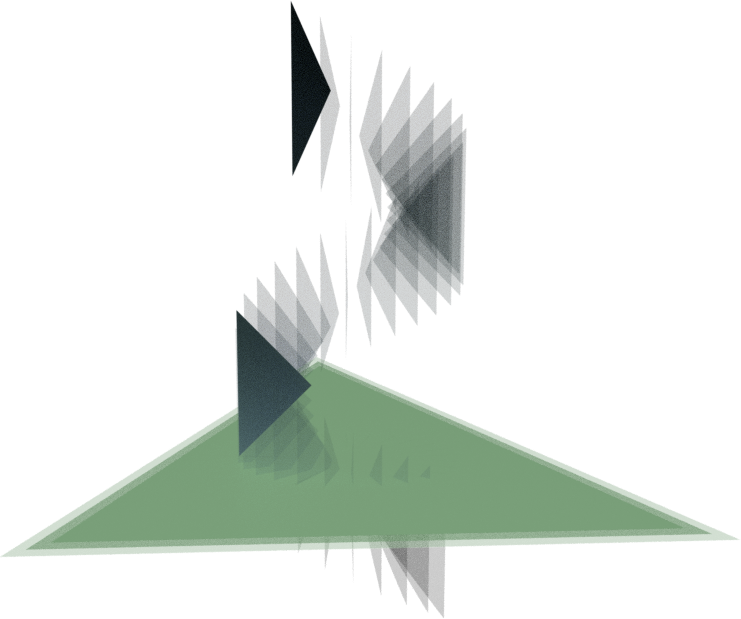
\includegraphics[width=0.8\linewidth]{fig/spiral.png}
	\caption{Test problem: \FS{caption}}
	\label{fig:tori}
\end{figure}
We consider the classical problem of continuous collision detection (CCD): given two primitives in space with some prescribed trajectory, we seek the first time in $[0,1]$ for which the primitives first come into contact, and call it $t^*$.
This type of test is essential in the simulation field to guarantee that physical objects do not interpenetrate.
In practice, finding the exact value of $t^*$ may be infeasible and often unnecessary. With interval methods, we instead seek an interval $T^*$ that is guaranteed to contain $t^*$ and is smaller than a user-specified precision $\delta>0$.
Then the lower bound of $T^*$ tells us a moment in time until which we can safely move the objects without collisions, and the upper bound gives a moment when a collision has surely happened already.
The difficulty of the query depends on the type of primitives, the type of trajectory, and the precision required.

Within MiSo, this is formulated as a \textsc{Minimize} problem, that is, a constrained global optimization \cite{Sichetti2025}.
In this case the optimization variables are $\{\mathbf{u}, \mathbf{v}, t\}$, where $\mathbf{u}=(u_0, u_1)$ and $\mathbf{v}=(v_0, v_1)$ are the parametric coordinates of the two primitives, and $t$ is time;
the constraints are the domain constraints $(u_0,u_1,v_0,v_1,t)\in[0,1]^5, u_0+u_1\leq1, v_0+v_1\leq1$ (which are all implicit in MiSo), and the collision constraint $d(x,y)<\epsilon$ with a small but positive $\epsilon$ -- i.e., we only consider pairs of points for which collision happens.
The objective function is $t$ -- i.e., we want to find the collision that happens earliest.

In our test, we consider two moving linear (i.e., flat) triangles, where one is linearly deforming (i.e., each vertex follows a linear trajectory independent of the others), while the other vertex is undergoing a rigid roto-translation, following a spiral motion.
More precisely, the center of the second triangle follows the spiral, and its normal remains aligned with the spiral's tangent. 
Of course, computing the roto-translation requires trigonometric functions, while all other computations involved are algebraic.

We test the same problem with different sets of parameters, changing the speed of the rotation and the position of the other triangle. The queries implemented with TIGHT take $27$ms, $133$ms and $2.5$s respectively, versus the $127$ms, $756$ms and $13.2$s of Filib++, for a speedup of approximately $5\times$.

\subsubsection{Intersection of two parametric tori}
\begin{figure}
	\centering
	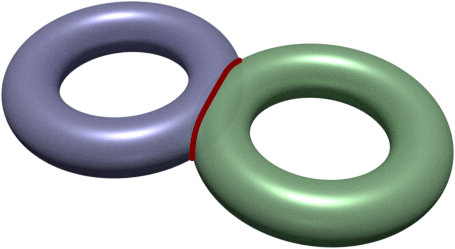
\includegraphics[width=0.8\linewidth]{fig/torusInt.png}
	\caption{Test problem: surface-surface intersection (SSI) of two parametric tori of inner radius $0.3$ and outer radius $1$, each shifted by $\pm1.1$ along the $x$ axis.}
	\label{fig:tori}
\end{figure}
Computing the intersection of parametric surfaces, also known as surface-surface intersection (SSI), is an important operation in CAD.
In our example, we want to describe the intersection locus of two tori expressed parametrically.
Again, the parametric representation of each torus requires computing trigonometric functions.

SSI can be formulated in MiSo as a \textsc{Solve} problem, that is, the problem of covering the set of all solutions of a constraint system within a certain tolerance.
Being a conservative method, the algorithm returns a region that is larger than the true solution, but is guaranteed to contain every point of it.

Similarly to the previous example, the optimization variables are $\{\mathbf{u}, \mathbf{v}\}$, where $\mathbf{u}=(u_0, u_1)$ and $\mathbf{v}=(v_0, v_1)$ are the parametric coordinates of the two tori;
the constraints are the domain constraints $(u_0,u_1,v_0,v_1)\in[0,1]^4$ (implicit in MiSo), and the intersection constraint $d(x,y)<\epsilon$.
This formulation gives solutions in \emph{parameter} space rather than physical space. To be precise, this formulation solves a more general version of the problem: since the parameter space is 4-dimensional, the solution is a collection of 4D boxes that describe pairs of contacting regions, up to the specified tolerance.

In both cases, the solver performs 11105 iterations and found a solution composed of 6976 4D boxes. However, the result took $136$ms to compute with TIGHT and $2186$ms with Filib++, a speedup of about $16\times$.

\subsection{Pathological cases}
Not producing tight enough intervals can have unpredictable results for seemingly easy problems. We provide a very simple example where returning a slightly larger interval results in the program being unable to compute the result.

\begin{figure}
	
\includegraphics[width=0.4\linewidth]{fig/512x512.png}
	\centering
	\caption{An example where tighter intervals of CR functions prevent errors: when the inputs to the problem are a few ULPs away from producing pathological situations, CR minimizes error and is often able to avoid failure. Moreover, its results are machine-independent; a non-CR implementation may complete successfully on one machine but fail on another.}
	\label{fig:tori}
\end{figure}
Suppose we have a function $f(x,y)$ defined on the plane that is inversely proportional to the distance of point $(x,y)$ to a circle centered in the origin with radius 5.
Thus, we are evaluating $f(x,y) = 1/(\sqrt{x^2 + y^2}-5)$.
This type of function resembles contact potentials used in IPC physical simulations \cite{Li2020IPC}.
We want to evaluate $f$ with interval arithmetic at point $P(3+10^{-15},4+10^{-15})$, so that $P$ lies outside the sphere. Remember that, because we are using interval arithmetic, we need not fear that adding a small value leads to cancellation for very small $\epsilon$: in those cases we simply get an interval that contains the true value.
We compute this function in three ways:
\begin{itemize}
	\item with TIGHT intervals, and using the function \texttt{hypot} to compute the Euclidean distance of $P$ from the origin (which is absent in Filib++);
	\item with TIGHT intervals, using only operators which are also supported by Filib++ (all algebraic in this case);
	\item with Filib++ intervals, using the same mode as the rest of the paper.
\end{itemize}
In the first two cases, the denominator is correctly computed as positive with TIGHT and the operation returns a real interval (albeit larger in the second case, due to multiple operations being involved).
When using Filib++, the square root produces an interval with lower bound equal to the radius, resulting in a division by zero.

While this example involves only a few operations, for more complex expressions, the propagation of error can be even more dramatic. 
While correct rounding does not eliminate the issue, it reduces propagation to a minimum and makes it predictable, since each operation can introduce at most 1 ULP of error on each side.

%\clearpage
\onecolumn
\begingroup

\tiny
\begin{longtable}{lrrrrrrrrr}
\hline
& Filib & Boost & FL++ NS & FL++ ND & FL++ NOG & FL++ Mul & FL++ PS & TIGHT & FP baseline \\
\hline
ADDITION & 139.841000 & 451.849000 & 77.454000 & 56.244000 & 16.264000 & 46.557000 & 58.725000 & 5.904000 & 5.912000 \\
SUBTRACTION & 135.853000 & 451.776000 & 77.444000 & 56.186000 & 16.295000 & 40.737000 & 58.831000 & 5.914000 & 5.911000 \\
MULTIPLICATION & 153.026000 & 454.497000 & 80.465000 & 58.602000 & 17.472000 & 64.090000 & 86.292000 & 11.230000 & 5.898000 \\
DIVISION & 148.818000 & 448.056000 & 98.105000 & 74.635000 & 37.021000 & 61.618000 & 82.163000 & 47.171000 & 11.826000 \\
SQUARE ROOT & 159.648000 & 447.951000 & 79.588000 & 63.828000 & 46.856000 & 60.580000 & 96.586000 & 35.396000 & 23.587000 \\
EXPONENTIAL & 257.656000 & 449.746000 & 254.173000 & 251.163000 & 205.657000 & 219.957000 & 246.876000 & 178.049000 & 57.764000 \\
SIN & 289.798000 & 1453.097000 & 327.376000 & 324.451000 & 207.906000 & 220.579000 & 233.763000 & 1971.934000 & 317.734000 \\
COS & 288.131000 & 1304.546000 & 324.974000 & 321.932000 & 207.339000 & 221.081000 & 230.165000 & 1943.731000 & 321.314000 \\
ARITHMETIC EXPRESSION 1 & 800.244000 & 2238.724000 & 569.425000 & 506.251000 & 229.616000 & 606.002000 & 757.993000 & 293.389000 & 58.910000 \\
ARITHMETIC EXPRESSION 2 & 1139.821000 & 3363.927000 & 718.223000 & 562.186000 & 175.775000 & 713.381000 & 863.089000 & 190.415000 & 47.126000 \\
ARITHMETIC EXPRESSION 3 & 1471.388000 & 4256.047000 & 998.436000 & 831.644000 & 458.746000 & 1124.630000 & 1325.309000 & 432.067000 & 70.696000 \\
ARITHMETIC EXPRESSION 4 & 3024.144000 & 9191.820000 & 1913.025000 & 1469.517000 & 585.462000 & 2044.504000 & 3184.462000 & 459.122000 & 94.246000 \\
ARITHMETIC EXPRESSION 5 & 2119.622000 & 6502.706000 & 1393.962000 & 1059.133000 & 367.301000 & 1411.076000 & 2217.277000 & 383.853000 & 94.231000 \\
ARITHMETIC EXPRESSION 6 & 1101.514000 & 3366.891000 & 687.291000 & 545.948000 & 158.213000 & 661.872000 & 883.903000 & 139.138000 & 23.585000 \\
ARITHMETIC EXPRESSION 7 & 727.897000 & 2243.477000 & 475.341000 & 359.346000 & 108.662000 & 401.904000 & 515.303000 & 142.828000 & 35.334000 \\
ARITHMETIC EXPRESSION 8 & 769.365000 & 2240.706000 & 501.354000 & 409.604000 & 128.150000 & 481.864000 & 564.428000 & 164.013000 & 35.331000 \\
ARITHMETIC EXPRESSION 9 & 3531.364000 & 10761.818000 & 2359.372000 & 1799.626000 & 699.956000 & 2391.969000 & 3727.499000 & 664.133000 & 164.909000 \\
ARITHMETIC EXPRESSION 10 & 1373.598000 & 4270.300000 & 907.073000 & 721.146000 & 199.894000 & 838.060000 & 1163.332000 & 237.028000 & 58.922000 \\
RANDOM EXPRESSION 1 & 1827.720000 & 6615.070000 & 1779.349000 & 1609.323000 & 1542.162000 & 1642.973000 & 1870.718000 & 6340.366000 & 1015.198000 \\
RANDOM EXPRESSION 2 & 1110.558000 & 1574.543000 & 1207.523000 & 1209.263000 & 1202.284000 & 1211.369000 & 1241.036000 & 789.165000 & 274.175000 \\
RANDOM EXPRESSION 3 & 2564.935000 & 9867.541000 & 2537.120000 & 2239.824000 & 1853.468000 & 2204.140000 & 2587.499000 & 8508.530000 & 1236.388000 \\
RANDOM EXPRESSION 4 & 2493.733000 & 9065.295000 & 2429.218000 & 2193.551000 & 1959.358000 & 2149.981000 & 2358.275000 & 7401.421000 & 1053.076000 \\
RANDOM EXPRESSION 5 & 4295.013000 & 18143.857000 & 4302.392000 & 3851.088000 & 3412.519000 & 3760.806000 & 4273.319000 & 16603.437000 & 3267.921000 \\
RANDOM EXPRESSION 6 & 7123.256000 & 32280.897000 & 6643.304000 & 6209.411000 & 4621.778000 & 5985.760000 & 7125.158000 & 29410.590000 & 5601.662000 \\
RANDOM EXPRESSION 7 & 3380.392000 & 11034.476000 & 3399.323000 & 3058.806000 & 2786.271000 & 3095.534000 & 3374.356000 & 11130.759000 & 1734.586000 \\
RANDOM EXPRESSION 8 & 1311.223000 & 4473.228000 & 1187.424000 & 1168.751000 & 1161.100000 & 1213.181000 & 1331.393000 & 6055.558000 & 1215.196000 \\
RANDOM EXPRESSION 9 & 3400.103000 & 10210.072000 & 3254.755000 & 3225.024000 & 3226.479000 & 3289.355000 & 3422.299000 & 11014.137000 & 1435.637000 \\
RANDOM EXPRESSION 10 & 4138.037000 & 17332.834000 & 4199.233000 & 3891.382000 & 2984.560000 & 3604.736000 & 4267.214000 & 18873.356000 & 2856.765000 \\
rigidBody2 & 1096.688000 & 3367.143000 & 633.011000 & 454.095000 & 151.639000 & 813.494000 & 830.272000 & 81.743000 & 12.110000 \\
triangle11 & 1339.602000 & 4491.835000 & 1060.539000 & 819.971000 & 275.963000 & 668.278000 & 906.220000 & 95.955000 & 23.643000 \\
sine & 1279.160000 & 4261.529000 & 893.492000 & 702.348000 & 388.753000 & 971.968000 & 1101.282000 & 116.442000 & 35.364000 \\
sum & 603.018000 & 2022.259000 & 344.715000 & 231.917000 & 28.484000 & 202.413000 & 306.228000 & 17.685000 & 13.274000 \\
test05nonlin1, r4 & 337.751000 & 1141.695000 & 232.326000 & 193.339000 & 41.939000 & 153.593000 & 178.452000 & 51.607000 & 12.886000 \\
hartman3 & 4712.450000 & 15262.228000 & 4173.571000 & 3395.213000 & 1697.997000 & 3611.646000 & 5104.652000 & 1064.881000 & 250.838000 \\
NMSE example 3.5 & 515.136000 & 1478.805000 & 491.804000 & 354.802000 & 277.643000 & 333.407000 & 445.790000 & 261.077000 & 120.126000 \\
Shoelace formula & 962.584000 & 2928.785000 & 534.187000 & 392.263000 & 138.700000 & 612.959000 & 720.627000 & 64.175000 & 14.922000 \\
NMSE example 3.10 & 551.913000 & 1348.582000 & 578.566000 & 420.741000 & 299.711000 & 376.984000 & 425.219000 & 815.674000 & 123.662000 \\
xbyxy & 202.976000 & 673.115000 & 156.073000 & 108.681000 & 37.741000 & 68.940000 & 122.748000 & 47.172000 & 11.819000 \\
NMSE section 3.11 & 594.957000 & 1129.898000 & 544.280000 & 533.606000 & 429.692000 & 500.523000 & 552.525000 & 342.734000 & 124.125000 \\
NMSE problem 3.3.1 & 393.005000 & 1138.265000 & 236.223000 & 185.712000 & 56.550000 & 185.663000 & 201.172000 & 24.311000 & 24.309000 \\
floudas2 & 138.222000 & 454.552000 & 77.722000 & 55.966000 & 16.183000 & 53.964000 & 58.758000 & 5.910000 & 5.893000 \\
test03nonlin2 & 274.542000 & 899.087000 & 201.572000 & 144.665000 & 41.662000 & 110.584000 & 143.203000 & 47.256000 & 11.801000 \\
nonlin2 & 518.287000 & 1793.875000 & 356.922000 & 277.021000 & 65.980000 & 302.369000 & 301.113000 & 58.751000 & 11.958000 \\
Complex sine and cosine & 874.427000 & 2574.310000 & 981.011000 & 848.995000 & 633.686000 & 734.288000 & 814.541000 & 2327.376000 & 401.627000 \\
floudas & 134.963000 & 451.753000 & 77.556000 & 56.111000 & 16.277000 & 32.403000 & 58.207000 & 5.916000 & 5.892000 \\
NMSE problem 3.4.2 & 1248.118000 & 3148.093000 & 1388.299000 & 1274.505000 & 756.863000 & 1107.437000 & 1240.167000 & 641.644000 & 177.688000 \\
NMSE example 3.8 & 743.097000 & 2019.136000 & 655.366000 & 609.324000 & 305.196000 & 453.241000 & 582.945000 & 812.049000 & 120.653000 \\
polarToCarthesian, x & 397.000000 & 1572.892000 & 466.554000 & 335.737000 & 223.962000 & 286.343000 & 323.319000 & 1016.368000 & 81.874000 \\
turbine1 & 1012.643000 & 3370.635000 & 644.964000 & 472.508000 & 116.244000 & 621.345000 & 680.219000 & 116.815000 & 24.217000 \\
triangle9 & 1337.699000 & 4491.263000 & 1059.422000 & 819.973000 & 275.852000 & 666.640000 & 895.069000 & 95.963000 & 23.669000 \\
sineOrder3 & 417.451000 & 1347.220000 & 233.925000 & 158.511000 & 25.356000 & 233.001000 & 291.788000 & 26.015000 & 5.934000 \\
doppler3 & 852.926000 & 2695.586000 & 512.794000 & 367.447000 & 67.302000 & 519.224000 & 509.392000 & 49.044000 & 11.826000 \\
triangle1 & 1343.976000 & 4491.789000 & 1064.973000 & 819.938000 & 276.008000 & 687.754000 & 896.190000 & 95.991000 & 23.654000 \\
NMSE p42, negative & 733.592000 & 2019.511000 & 474.269000 & 397.573000 & 134.240000 & 467.709000 & 532.497000 & 96.133000 & 30.116000 \\
matrixDeterminant2 & 1335.914000 & 4037.783000 & 768.697000 & 590.954000 & 291.377000 & 994.170000 & 1151.122000 & 127.204000 & 17.702000 \\
delta & 2363.775000 & 8071.711000 & 1487.744000 & 1069.958000 & 368.422000 & 1623.485000 & 2516.267000 & 201.618000 & 35.574000 \\
test06sums4, sum1 & 276.214000 & 899.933000 & 154.370000 & 109.818000 & 16.670000 & 70.498000 & 116.089000 & 5.911000 & 6.271000 \\
sec4-example & 510.909000 & 1792.815000 & 358.227000 & 276.106000 & 64.924000 & 291.070000 & 299.062000 & 58.110000 & 11.850000 \\
logexp & 571.539000 & 900.015000 & 429.090000 & 422.216000 & 406.535000 & 470.908000 & 523.480000 & 608.036000 & 101.801000 \\
NMSE problem 3.3.5 & 613.752000 & 2814.852000 & 654.772000 & 640.610000 & 411.896000 & 474.869000 & 534.066000 & 3917.989000 & 645.331000 \\
NMSE example 3.3 & 624.144000 & 3115.015000 & 659.109000 & 644.230000 & 420.507000 & 481.649000 & 535.004000 & 3984.539000 & 639.393000 \\
kepler0 & 934.094000 & 3374.042000 & 591.144000 & 410.800000 & 96.445000 & 446.641000 & 690.757000 & 68.643000 & 12.998000 \\
triangle5 & 1330.043000 & 4491.454000 & 1054.046000 & 819.945000 & 275.962000 & 679.206000 & 897.956000 & 95.985000 & 23.634000 \\
bspline3 & 349.558000 & 896.634000 & 170.890000 & 132.328000 & 23.763000 & 149.554000 & 151.591000 & 25.208000 & 11.814000 \\
predatorPrey & 517.708000 & 1797.241000 & 362.751000 & 264.453000 & 71.540000 & 295.467000 & 315.223000 & 75.174000 & 23.547000 \\
turbine3 & 1078.464000 & 3374.784000 & 657.901000 & 473.523000 & 115.918000 & 671.678000 & 731.489000 & 120.067000 & 24.374000 \\
triangle7 & 1333.909000 & 4491.519000 & 1060.567000 & 820.037000 & 275.935000 & 678.737000 & 904.532000 & 95.977000 & 23.640000 \\
doppler1 & 856.010000 & 2694.662000 & 512.790000 & 367.413000 & 67.356000 & 511.259000 & 508.052000 & 49.022000 & 11.824000 \\
triangle3 & 1343.285000 & 4491.633000 & 1059.280000 & 820.024000 & 275.915000 & 675.874000 & 895.355000 & 95.984000 & 23.662000 \\
Rump's example, C & 2473.162000 & 8509.362000 & 1663.972000 & 1315.420000 & 759.647000 & 2049.098000 & 2535.792000 & 133.600000 & 18.490000 \\
exp1x & 419.860000 & 898.201000 & 472.654000 & 303.216000 & 233.508000 & 308.834000 & 361.977000 & 173.688000 & 52.859000 \\
NMSE problem 3.4.4 & 815.684000 & 1799.601000 & 753.586000 & 631.378000 & 563.758000 & 689.865000 & 822.923000 & 388.001000 & 141.606000 \\
delta4 & 1133.072000 & 3824.396000 & 680.522000 & 464.514000 & 100.704000 & 603.177000 & 910.545000 & 84.924000 & 14.717000 \\
instantaneousCurrent & 4488.761000 & 16970.875000 & 4069.743000 & 3347.207000 & 1772.621000 & 3921.790000 & 4572.856000 & 3542.066000 & 249.317000 \\
NMSE problem 3.2.1, negative & 580.000000 & 1575.099000 & 391.866000 & 343.297000 & 141.013000 & 366.826000 & 388.945000 & 95.234000 & 30.114000 \\
kepler2 & 2253.051000 & 8074.229000 & 1476.404000 & 1055.691000 & 299.644000 & 1350.289000 & 2307.827000 & 202.517000 & 31.426000 \\
NMSE problem 3.3.3 & 596.981000 & 1801.427000 & 388.592000 & 272.221000 & 84.582000 & 291.734000 & 353.846000 & 36.415000 & 36.155000 \\
azimuth & 2280.088000 & 9580.675000 & 2244.388000 & 1913.964000 & 1623.961000 & 1893.445000 & 2035.415000 & 7440.727000 & 557.777000 \\
NMSE problem 3.3.7 & 598.215000 & 1131.234000 & 612.145000 & 515.712000 & 410.170000 & 490.731000 & 563.524000 & 356.303000 & 126.512000 \\
i6 & 348.473000 & 1647.079000 & 341.872000 & 337.572000 & 222.369000 & 243.379000 & 287.750000 & 1633.076000 & 85.102000 \\
NMSE example 3.9 & 552.721000 & 1726.968000 & 596.867000 & 556.534000 & 289.913000 & 391.215000 & 460.772000 & 1264.309000 & 339.103000 \\
NMSE section 3.5 & 398.016000 & 898.768000 & 486.733000 & 303.016000 & 245.139000 & 300.453000 & 367.014000 & 197.396000 & 55.691000 \\
hypot & 342.477000 & 1122.022000 & 263.823000 & 238.321000 & 91.797000 & 224.506000 & 236.291000 & 47.483000 & 23.592000 \\
test04dqmom9 & 2386.646000 & 7176.255000 & 1458.446000 & 1147.777000 & 541.147000 & 1792.461000 & 2241.113000 & 222.694000 & 36.870000 \\
nonlin1 & 204.094000 & 673.566000 & 154.107000 & 108.823000 & 37.646000 & 68.386000 & 122.449000 & 47.215000 & 11.817000 \\
NMSE example 3.4 & 664.564000 & 2980.073000 & 661.015000 & 624.384000 & 435.720000 & 515.363000 & 550.968000 & 3860.527000 & 631.596000 \\
hartman6 & 8441.579000 & 28732.496000 & 6675.589000 & 5234.865000 & 2195.664000 & 6219.582000 & 9146.217000 & 1425.817000 & 312.680000 \\
carthesianToPolar, radius & 340.186000 & 1122.005000 & 262.460000 & 239.171000 & 87.975000 & 199.452000 & 216.425000 & 47.469000 & 23.595000 \\
triangle & 1355.984000 & 4491.370000 & 1064.677000 & 819.935000 & 275.928000 & 691.038000 & 901.196000 & 96.010000 & 23.636000 \\
jetEngine & 4359.431000 & 14353.908000 & 2896.103000 & 2259.655000 & 961.222000 & 3185.314000 & 4501.869000 & 290.648000 & 32.992000 \\
sqroot & 944.149000 & 3370.391000 & 612.010000 & 432.251000 & 109.613000 & 635.199000 & 590.473000 & 91.940000 & 16.391000 \\
triangle12 & 1343.855000 & 4491.469000 & 1062.189000 & 819.967000 & 275.913000 & 668.453000 & 923.339000 & 95.945000 & 23.652000 \\
triangle10 & 1343.627000 & 4491.394000 & 1060.932000 & 819.955000 & 275.905000 & 657.708000 & 895.633000 & 96.001000 & 23.668000 \\
turbine2 & 787.646000 & 2468.374000 & 485.223000 & 355.833000 & 83.628000 & 523.906000 & 568.031000 & 92.648000 & 13.073000 \\
triangle2 & 1349.661000 & 4491.501000 & 1060.174000 & 819.947000 & 275.856000 & 658.290000 & 889.431000 & 96.068000 & 23.639000 \\
rigidBody1 & 499.257000 & 1571.369000 & 277.324000 & 192.437000 & 33.012000 & 275.614000 & 295.456000 & 27.934000 & 6.714000 \\
NMSE problem 3.4.1 & 499.820000 & 1935.497000 & 495.778000 & 445.141000 & 234.839000 & 348.744000 & 393.001000 & 1937.419000 & 323.871000 \\
exp1xlog & 861.737000 & 1372.868000 & 839.657000 & 669.773000 & 658.511000 & 719.369000 & 771.246000 & 768.945000 & 176.738000 \\
Complex square root & 677.775000 & 2022.524000 & 478.818000 & 448.335000 & 193.064000 & 444.889000 & 523.104000 & 80.550000 & 40.673000 \\
carthesianToPolar, theta & 369.999000 & 1063.295000 & 478.198000 & 270.977000 & 190.656000 & 240.149000 & 286.038000 & 395.114000 & 67.595000 \\
NMSE example 3.7 & 346.028000 & 673.768000 & 269.469000 & 263.258000 & 215.692000 & 254.656000 & 307.312000 & 181.984000 & 55.634000 \\
floudas3 & 446.175000 & 1347.691000 & 232.976000 & 156.858000 & 23.549000 & 211.433000 & 264.065000 & 17.055000 & 5.896000 \\
NMSE example 3.6 & 575.899000 & 1571.854000 & 408.961000 & 383.614000 & 149.620000 & 336.309000 & 363.886000 & 94.401000 & 61.769000 \\
i4 & 306.219000 & 899.382000 & 225.286000 & 131.355000 & 51.645000 & 127.900000 & 197.492000 & 36.702000 & 23.587000 \\
test02sum8 & 553.056000 & 1797.845000 & 304.836000 & 208.652000 & 25.876000 & 173.014000 & 289.805000 & 11.815000 & 11.782000 \\
triangle6 & 1340.512000 & 4491.380000 & 1065.315000 & 819.995000 & 275.932000 & 684.508000 & 897.417000 & 96.035000 & 23.652000 \\
carbonGas & 633.969000 & 2063.988000 & 394.711000 & 292.047000 & 72.406000 & 296.220000 & 461.252000 & 42.795000 & 13.133000 \\
sphere & 708.084000 & 3291.394000 & 668.765000 & 637.000000 & 393.829000 & 551.753000 & 617.975000 & 2053.451000 & 116.283000 \\
test01sum3 & 600.117000 & 2022.147000 & 344.752000 & 231.906000 & 28.469000 & 196.147000 & 289.398000 & 17.683000 & 13.268000 \\
test05nonlin1, test2 & 208.727000 & 678.465000 & 155.104000 & 109.365000 & 38.017000 & 73.359000 & 124.173000 & 11.770000 & 11.786000 \\
kepler1 & 1534.837000 & 5387.201000 & 965.331000 & 696.391000 & 166.707000 & 946.730000 & 1624.203000 & 118.510000 & 20.213000 \\
NMSE example 3.1 & 424.877000 & 1122.665000 & 247.424000 & 167.236000 & 123.937000 & 238.997000 & 232.539000 & 71.246000 & 37.569000 \\
matrixDeterminant & 1306.568000 & 4040.408000 & 768.910000 & 590.688000 & 276.258000 & 997.373000 & 1157.617000 & 124.680000 & 17.704000 \\
NMSE p42, positive & 717.345000 & 2019.561000 & 472.198000 & 389.439000 & 127.389000 & 469.201000 & 518.698000 & 96.015000 & 30.050000 \\
sqrtadd & 506.413000 & 1346.585000 & 319.466000 & 249.144000 & 128.995000 & 274.941000 & 296.415000 & 84.254000 & 47.154000 \\
NMSE problem 3.4.5 & 792.389000 & 2993.750000 & 876.489000 & 749.898000 & 479.788000 & 570.157000 & 642.935000 & 3235.422000 & 652.276000 \\
floudas1 & 1675.451000 & 5614.112000 & 1050.390000 & 748.274000 & 209.619000 & 1028.023000 & 1754.377000 & 90.824000 & 15.432000 \\
NMSE problem 3.3.2 & 748.989000 & 2504.716000 & 764.071000 & 752.515000 & 509.868000 & 551.905000 & 633.419000 & 2533.860000 & 652.241000 \\
intro-example & 202.243000 & 673.536000 & 154.102000 & 108.846000 & 37.650000 & 79.441000 & 122.476000 & 47.209000 & 11.798000 \\
test06sums4, sum2 & 282.668000 & 899.772000 & 154.919000 & 109.534000 & 17.039000 & 71.091000 & 110.263000 & 5.907000 & 6.622000 \\
himmilbeau & 1079.656000 & 3603.857000 & 661.332000 & 475.050000 & 137.398000 & 599.288000 & 990.714000 & 60.156000 & 8.686000 \\
NMSE problem 3.3.6 & 532.307000 & 1122.233000 & 425.726000 & 354.958000 & 277.861000 & 337.198000 & 404.582000 & 823.688000 & 120.724000 \\
intro-example-mixed & 212.109000 & 673.567000 & 154.098000 & 108.777000 & 37.672000 & 80.346000 & 122.445000 & 47.209000 & 11.787000 \\
NMSE problem 3.4.3 & 384.190000 & 1123.837000 & 497.130000 & 442.214000 & 227.765000 & 282.040000 & 348.713000 & 411.277000 & 58.651000 \\
exp1x32 & 419.900000 & 897.561000 & 475.516000 & 303.253000 & 233.530000 & 308.849000 & 362.038000 & 173.226000 & 52.684000 \\
NMSE problem 3.2.1, positive & 556.059000 & 1574.704000 & 392.185000 & 344.205000 & 123.767000 & 356.350000 & 381.967000 & 95.345000 & 30.066000 \\
polarToCarthesian, y & 403.183000 & 1733.631000 & 467.434000 & 339.948000 & 226.865000 & 283.291000 & 324.764000 & 1011.146000 & 81.761000 \\
Rump's example, FP & 2309.869000 & 7614.761000 & 1495.628000 & 1183.428000 & 651.137000 & 1936.570000 & 2352.014000 & 149.952000 & 18.556000 \\
triangle8 & 1347.005000 & 4491.694000 & 1058.567000 & 819.899000 & 275.912000 & 658.487000 & 895.219000 & 95.900000 & 23.666000 \\
verhulst & 350.615000 & 1121.993000 & 236.814000 & 190.891000 & 47.872000 & 117.664000 & 181.299000 & 64.693000 & 23.553000 \\
triangle4 & 1348.819000 & 4492.027000 & 1060.792000 & 819.955000 & 275.959000 & 660.079000 & 889.145000 & 96.004000 & 23.682000 \\
doppler2 & 844.834000 & 2695.186000 & 514.055000 & 367.496000 & 67.403000 & 530.879000 & 524.273000 & 49.006000 & 11.800000 \\
\hline
\end{longtable}

\endgroup
\clearpage
\twocolumn


%\section{Conclusions and future work}
We have introduced TIGHT, an efficient C++ library for correctly rounded interval arithmetic built on top of the state-of-the art in both correctly rounded computations and interval arithmetic.

The authors are committed to making TIGHT a usable piece of software: unlike a large share of other related libraries, TIGHT can be easily integrated into CMake projects. Its source code is available at \url{url://omitted.for.anonimity}.

TIGHT is designed to be future-proof: if correctly rounded mathematical routines become the standard in the coming years, or a more performant CR methodologies are developed, switching the underlying library requires minimal changes.
Crucially, since the result of a CR operation is well defined, TIGHT will continue to return the same results \emph{forever} on all machines, even in the event of a library change (the only exception to this is, of course bug fixes).

The library could still be improved in several ways:
\begin{enumerate}
	\item NFG's arithmetic operations owe their speed to vectorization. Vectorized mathematical libraries exist \cite{sleef} but we are not aware of a correctly-rounded solution. In any case, having a non-CR, faster interval routines could still be useful for applications that can cope with error and inconsistencies across machines.
	\item TIGHT currently does not conform with the IEEE 1788-2015 standard for interval arithmetic \cite{ieee1788}. Adding compliance and testing with a framework such as \ref{Benet23} would make the library more easily integrated. This includes adding conformant support for infinity and NaN values.
	\item As mentioned in section \ref{}, integrating CR functions for multiplication with a real constant value as in \cite{crpi} would bring a more consistent speed for $\sin$ and $\cos$ on arbitrary arguments.
	\item CORE-MATH also contains a CR implementation of the gamma function (included in the C++ standard library), that could be used to build an interval implementation, though it is not clear whether this would be useful in practice.
\end{enumerate}


%-------------------------------------------------------------------------
% bibtex
\bibliographystyle{eg-alpha-doi}
\bibliography{biblio}


\end{document}
